In this section we explain how to use the simulator and how some simulations influenced the design of the robot.

\section{Simulation setup}
The basic idea is to use V-Rep as a simulation platform and use TCP/IP to have another program control the simulation from outside. This gives us great implementation flexibility and we can substitute the real robot by the simulation model easily. This is represented on \cref{fig:simulation_principles}. For this thesis, the control code will be written in MATLAB. 

\begin{figure}[htp]
\center
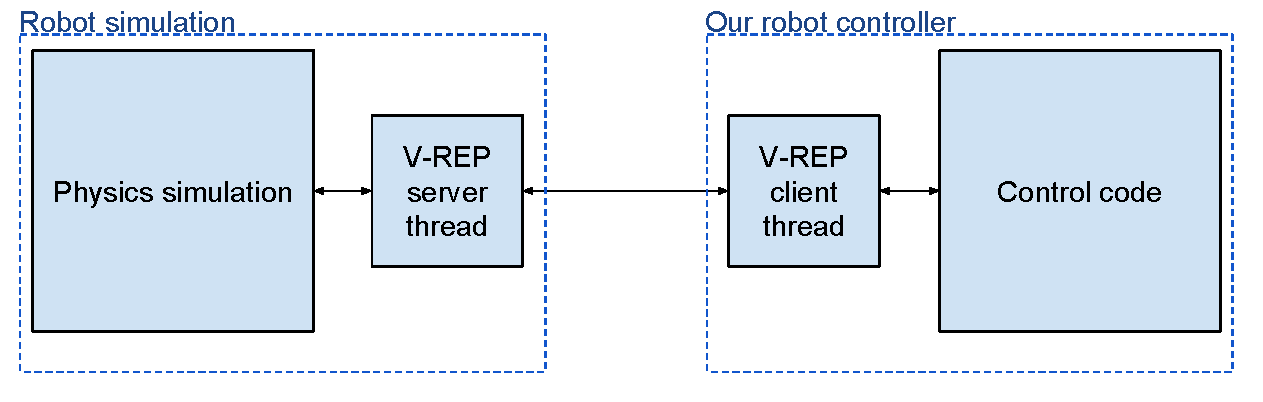
\includegraphics[width=0.6\textwidth]{figures/simulation_principles}
\caption[Simulation principles]{V-Rep simulates the robot while an external program sends order to the robot over TCP/IP thanks to the client/server thread provided by V-Rep.}
\label{fig:simulation_principles}
\end{figure}

Furthermore, the simulation will operate in the synchronous operation mode. That is, each simulation timestep must be triggered by the control code, allowing precise control of the robot. \Cref{fig:remoteApi} presents how V-Rep and the control code interact in synchronous mode.

\begin{figure}[htp]
\center
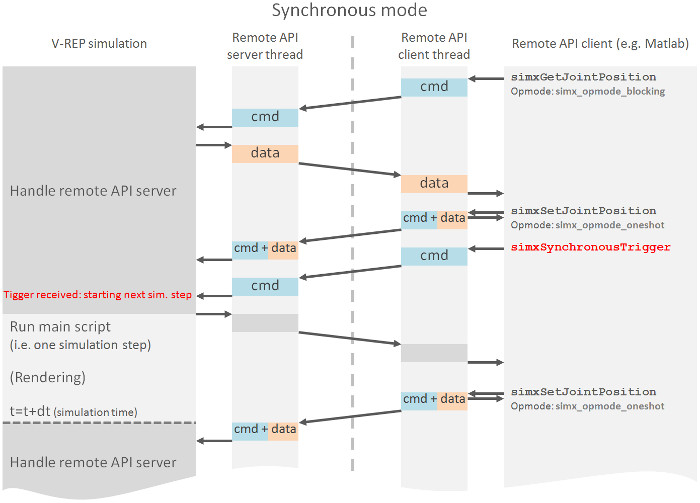
\includegraphics[width=0.6\textwidth]{figures/remoteApiSynchronous}
\caption[Simulation interaction]{Typical interaction between the simulator and the control code. The simulation runs on two threads : the simulation and the server thread. The server threads can receive orders from a client thread which is controlled by a custom application of our own. The simulator waits for a trigger before simulating the next timestep.}
\label{fig:remoteApi}
\end{figure}

\begin{lstlisting}[language=MATLAB, tabsize = 4, float, caption=Basic control program in MATLAB, captionpos = b, frame=leftline, keywordstyle=\color{blue}, numbers = left, commentstyle= \color{mygreen}]
function simulation_client_vrep()
dt = .01;

disp('Program started');
vrep = remApi('remoteApi');
vrep.simxFinish(-1); % close all opened connections
clientID = vrep.simxStart('127.0.0.1', 19997, true, true, 5000, 5);

if clientID < 0
    disp('Failed connecting to remote API server. Exiting.');
    vrep.delete();
    return;
end
disp('Connected to remote API server');

% We close the connexion whenever the script is interrupted.
cleanupObj = onCleanup(@() cleanup_vrep(vrep, clientID));

% This will only work in "continuous remote API server service"
vrep.simxSynchronous(clientID, true);

% retrieve handles to servos, joints
h = robot_init(vrep, clientID);

vrep.simxStartSimulation(clientID, vrep.simx_opmode_oneshot_wait);

i = 1;
while true && t < 3
    instructions = standup_prone(h, t);
    
    i = i + 1;
    send_instructions(vrep, clientID, instructions);
    t = t + dt;
end

% Before closing the connection to V-REP, make sure that the last command sent out had time to arrive.
vrep.simxGetPingTime(clientID);

% Now close the connection to V-REP:
vrep.simxStopSimulation(clientID, vrep.simx_opmode_oneshot_wait);
vrep.simxFinish(clientID);
vrep.delete(); % call the destructor!
disp('Program ended');
end

end
\end{lstlisting}

\section{Applications}
\subsection{Static stability}
The first application is simply to build a model of the robot and test if it is able to stand upright on its own.

The modelling begins in Blender where pieces are simplified/made convex and placed to create the structure of the robot. The model is then exported (in COLLADA) and imported into V-Rep. 

The feet are approximated by a thicker block in order to help with the collision detection. They are also given a high friction.

The torque of the servos is computed from the maximal torque of the DC motor and the reduction ratio of the gears. 
\begin{align*}
Torque &= TorqueMotor \times ReductionRatio\\
&= 3.67e^{-3} \times 193\\
&= 0.7083Nm
\end{align*}
In \cref{sec:exp1} we determined that the maximum torque the servo was actually able to produce was $1.7Nm$ so to represent this we choose to set the maximum torque of the servos to $1Nm$.

In V-Rep the different elements of the robot are dynamically enabled and given mass, accordingly to the values listed in \cref{table:weights}. Then, joints (motor controlled with control loop activated) are added to simulate the behaviour of the servos. Their maximal torque is set to $1.6$, the maximum torque developed my Mx-28 servos as shown by our earlier experiments (\cref{table:exp1_results}). 

\begin{table}[htp]
\center
\begin{tabularx}{\textwidth}{@{} l X X l @{}}
\toprule
\textbf{Module} & \textbf{Weight [$g$]} &  \textbf{Density [$kg/m^3$]}& \textbf{Dimensions [$mm \times mm \times mm$]}\\ 
\midrule
Odroid C-2 & 40 &  & 85.0 x 56.0 x 10.0\\
Li-Po battery & 188 & 2304 & 103.0 x 33.0 x 24.0\\
Mx-28R & 72 & 1150 & 35.6 x 50.6 x 35.5\\
LI-USB30-M021C & 22 & 2200 & 26.0 x 26.0 x 14.7\\
Frame Fr-07 & & 1200 & \\
Frame Fr-101-H3 & 7 & 1200 & \\
\bottomrule
\end{tabularx}
\caption[Weights and dimensions of the pieces of the robot]{Weights and dimensions of the pieces of the robot. The density is useful for the automatic computation of the weight and inertia of the pieces in V-REP.}
\label{table:weights}
\end{table}

The springs on the leg are simulated by two spherical joints and one prismatic joint set to spring-damper mode.

The servos of the robot are simply ordered to hold their initial angle and the simulation determines that the robot can indeed stand upright without any active stabilization.

\subsection{Standing up routines}
This section is heavily inspired by \cite{Stuckler06}

\subsection{Walking}

\section{Influence on robot's design}
The simulator helped shape the robot through simulations that unveiled serious design problems (inability to stand after a fall, inability to walk).

The first design is visible on \cref{fig:first_robot}. It was plagued by stability problems, overcomplicated arms and simulation difficulties. 
\begin{figure}[htp]
\center
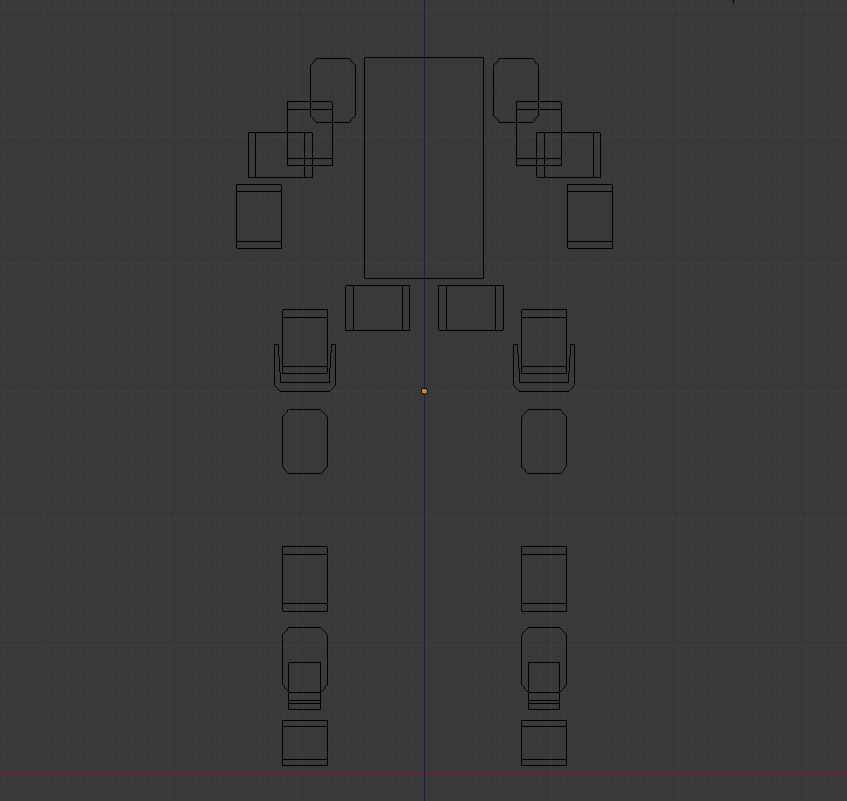
\includegraphics[width=0.6\textwidth]{figures/robot1}
\caption[Initial robot design]{First robot design. Arms use 4 servos each, making it quite heavy.}
\label{fig:first_robot}
\end{figure}

The final design, visible on \cref{fig:final_robot} has better stability, wider movement possibilities and can stand up and walk more easily. 
\begin{figure}[htp]
\center
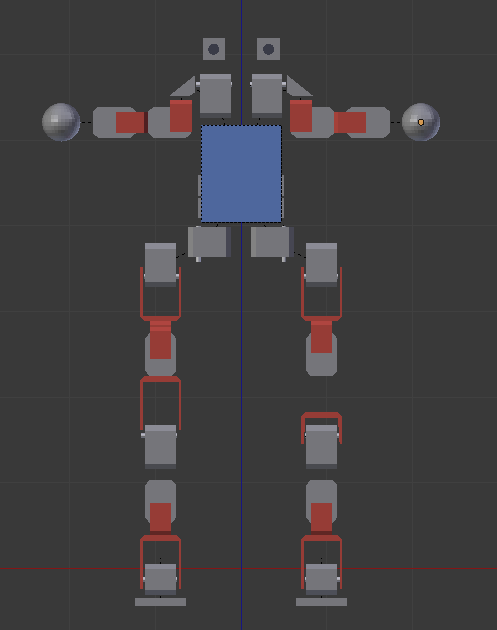
\includegraphics[width=0.6\textwidth]{figures/robot2}
\caption[Final robot design]{Final robot design. Arms now use 3 servos. The feet and the hips use a different configuration to have wider movement possibilities and bring down the center of gravity.}
\label{fig:final_robot}
\end{figure}

The final dimensions of the robot respect the rules of the contest:
\begin{itemize}
\item Height : $61.3cm$
\item Height of COM : $34cm$
\item Height of legs : $cm$
\item Height max is $< 1.5 \times 61.3$.
\item Foot area is $ cm^2$.
\end{itemize}